\documentclass[letterpaper,10pt,titlepage]{article}
\usepackage[letterpaper,margin=0.7in]{geometry}
\usepackage{tikz} \tikzset{>=latex}
\usepackage{pgfplots,tikz}
\usetikzlibrary{decorations.markings,arrows, calc, angles, quotes, decorations.pathmorphing,patterns, decorations.pathreplacing}
\pgfplotsset{compat=newest}
\usepackage{enumitem}
\usepackage{mathtools}
\mathtoolsset{showonlyrefs}
\usepackage{amssymb}
\usepackage{gensymb}
\usepackage{empheq}
\newcommand*\widefbox[1]{\fbox{\hspace{2em}#1\hspace{2em}}}
\usepackage{pdfpages}
\pagenumbering{gobble}
\newcommand{\itemn}{\newpage \setcounter{equation}{0} \item}
\usepackage{bm}
\usepackage{mathtools}
\usepackage{amsmath}
\usepackage{esint}
\usepackage{dirtytalk}
\usepackage{mathcomp}
\usepackage{mdframed}
\usepackage[pdfpagelabels]{hyperref}
%\begin{mdframed}[backgroundcolor=gray!20]
%\vspace{6pt}
%\end{mdframed}
\usepackage[margin=0.5in]{caption} %Allows for use of \caption* for non-labeled captions
\usepackage{graphicx}
\newcommand{\Lagr}{\mathcal{L}}
\graphicspath{ {images/} }
\usepackage{fancyhdr}

\newcommand{\infinitesum}[2]{\sum_{#1 = #2}^{\infty}}
\newcommand{\goodprime}{^{\prime}}
\newcommand{\tsi}[1]{\int_{\phi=0}^{2\pi}\int_{\theta=0}^{\pi}\int_{r=0}^{#1}}
\newcommand{\functionof}[2]{#1\left(#2\right)}
\newcommand{\unit}[1]{\,\hat{\bm{#1}}}
\newcommand{\vect}[1]{\mathbf{#1}}
\newcommand{\paren}[1]{\left(#1\right)}
\newcommand{\brackets}[1]{\left[#1\right]}
\newcommand{\abs}[1]{\left|#1\right|}
\newcommand{\eval}[3]{\left.#1\right|_{#2}^{#3}}
\newcommand{\anglers}[1]{\langle #1 \rangle}
\newcommand{\sinp}[1]{\sin{\paren{#1}}}
\newcommand{\cosp}[1]{\cos{\paren{#1}}}
\newcommand{\tanp}[1]{\tan{\paren{#1}}}

\newcommand{\sinpR}[2]{\sin^{#2}{\paren{#1}}}
\newcommand{\cospR}[2]{\cos^{#2}{\paren{#1}}}
\newcommand{\tanpR}[2]{\tan^{#2}{\paren{#1}}}


\newcommand{\expp}[1]{\exp\paren{#1}}
\newcommand{\thefrac}{\dfrac{n\pi}{d}}
\newcommand{\assolegendre}[1]{P_{#1}\paren{\cos{\theta}}}

\newcommand{\partialwoa}[1]{\dfrac{\partial}{\partial #1}}
\newcommand{\partiald}[2]{\dfrac{\partial}{\partial #2}\brackets{#1}}
\newcommand{\partialdd}[2]{\dfrac{\partial^2}{\partial^2 #2}\brackets{#1}}
\newcommand{\derivative}[2]{\dfrac{d #1}{d #2}}
\newcommand{\integral}[2]{\int_{#1}^{#2}}

\newcommand{\sn}[2]{#1\times10^{#2}}

%\begin{mdframed}[backgroundcolor=gray!20]
%\vspace{6pt}
%\end{mdframed}

\newcommand{\homeworkTitle}{Lab 09}
\newcommand{\homeworkDueDate}{November 26, 2018}
\newcommand{\homeworkClass}{MATH 3180}
\newcommand{\className}{Numerical Analysis}
\newcommand{\homeworkClassInstructor}{Dr. Seo}
\newcommand{\homeworkAuthorName}{Jackson Cole}

\title{\homeworkTitle\\
\homeworkClass: \className}
\author{\homeworkAuthorName}
\date{\homeworkDueDate}


\begin{document}
\maketitle
\tableofcontents
% The following makes equations look much nicer
\setlength{\abovedisplayskip}{10pt}
\setlength{\belowdisplayskip}{10pt}
\setlength{\abovedisplayshortskip}{10pt}
\setlength{\belowdisplayshortskip}{10pt}
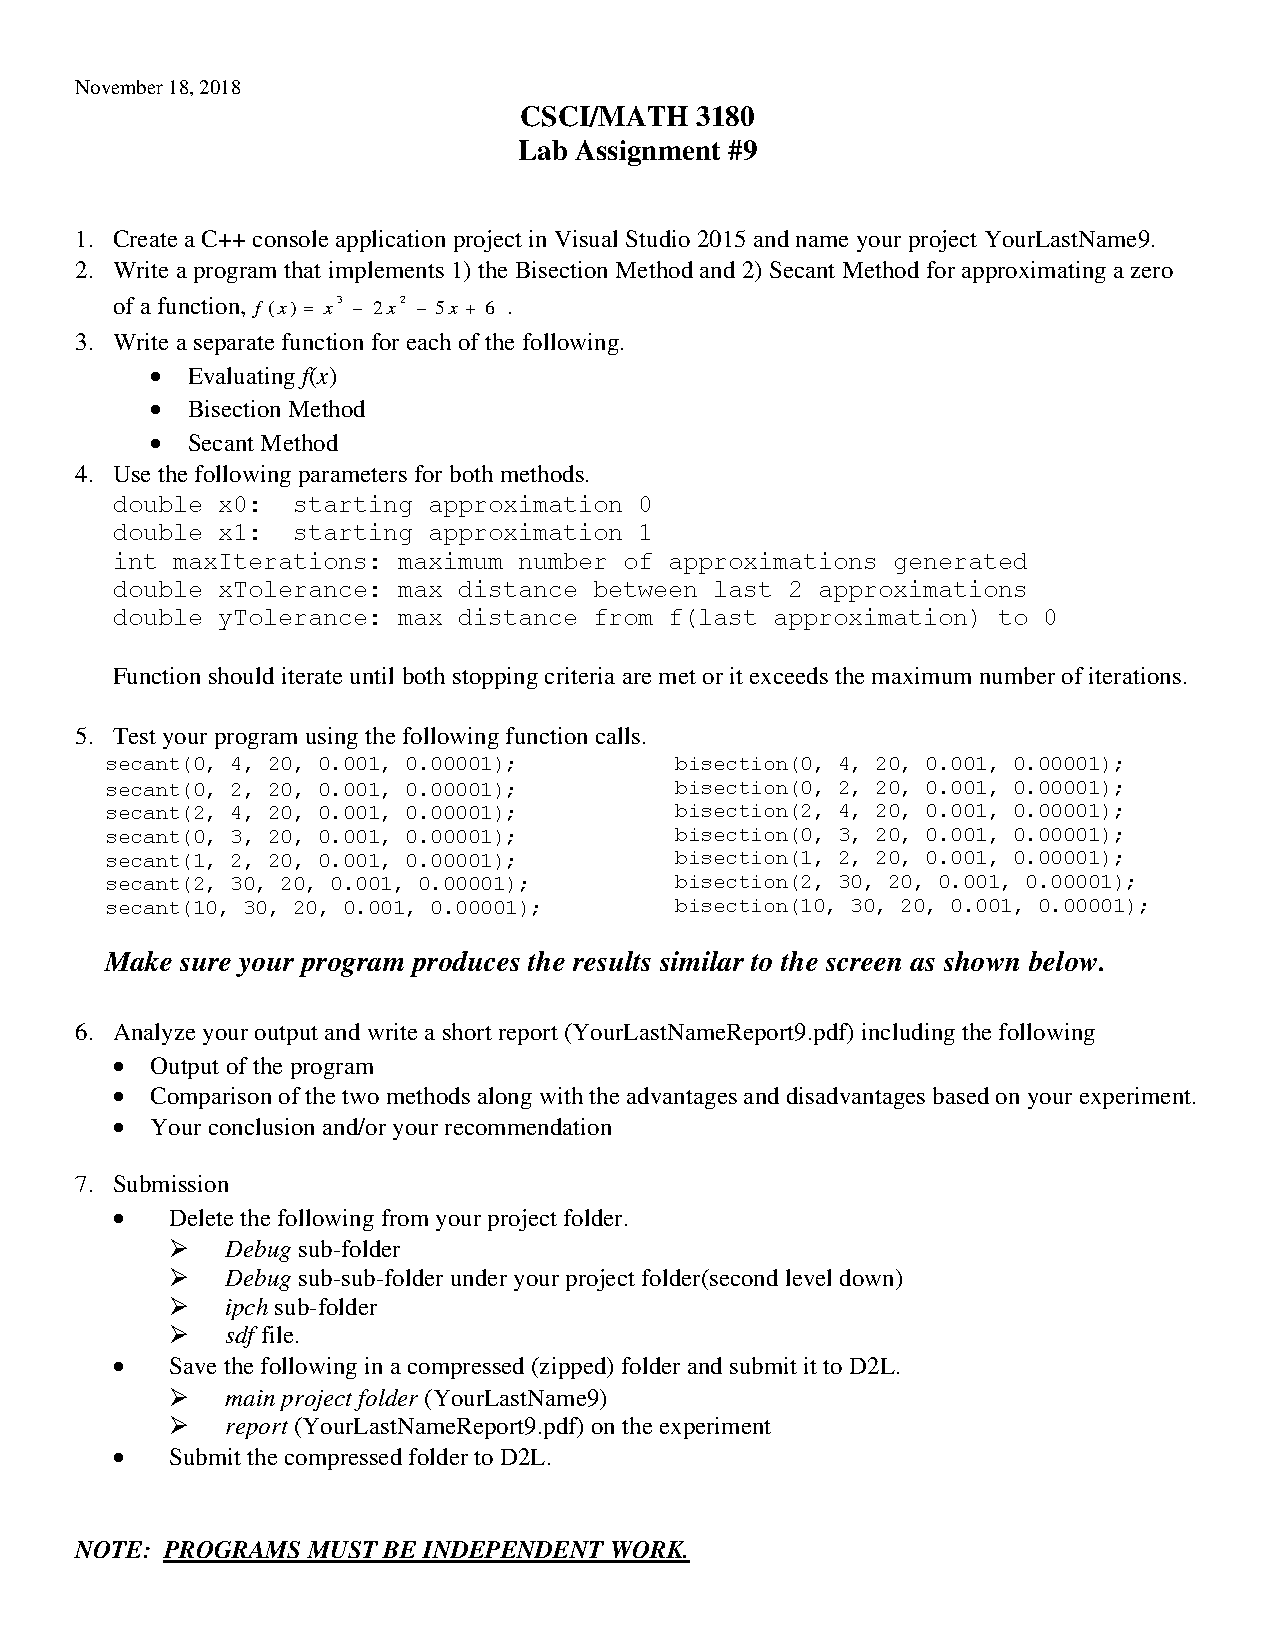
\includepdf[pages=-]{content/intropages-lab9.pdf}
\topmargin=-0.45in
\headsep=0.25in

\pagestyle{fancy}
\rhead{\homeworkAuthorName}
\chead{\homeworkClass\ (\homeworkClassInstructor): \homeworkTitle}

\section{Program Output}
\begin{verbatim}
####################################################################################################
Interval: [0.000000, 4.000000]
Secant Method
--------------------------------------------------------------------------------
   Iteration    Approximate Root             x_error             y_error
--------------------------------------------------------------------------------
           1           -2.000000            6.000000            0.000000
	Exact root found at -2.000000
	Number of iterations: 1


Interval: [0.000000, 4.000000]
Bisection Method
	Found no root on the interval


####################################################################################################
Interval: [0.000000, 2.000000]
Secant Method
--------------------------------------------------------------------------------
   Iteration    Approximate Root             x_error             y_error
--------------------------------------------------------------------------------
           1            1.200000            0.800000            1.152000
           2            0.876404            0.323596            0.754961
           3            1.004515            0.128111            0.027070
           4            1.000081            0.004435            0.000483
           5            1.000000            0.000081            0.000000
	Approximated root: 1.000000
	Number of iterations: 5
	x_error: 0.000081
	y_error: 0.000000


Interval: [0.000000, 2.000000]
Bisection Method
--------------------------------------------------------------------------------
   Iteration    Approximate Root             x_error             y_error
--------------------------------------------------------------------------------
           1            1.000000            2.000000            0.000000
	Exact root found at 1.000000
	Number of iterations: 1


####################################################################################################
Interval: [2.000000, 4.000000]
Secant Method
--------------------------------------------------------------------------------
   Iteration    Approximate Root             x_error             y_error
--------------------------------------------------------------------------------
           1            2.363636            1.636364            3.786627
           2            2.648045            0.284408            2.696043
           3            3.351133            0.703089            4.417689
           4            2.914509            0.436624            0.804372
           5            2.981764            0.067255            0.180039
           6            3.001158            0.019394            0.011591
           7            2.999985            0.001173            0.000149
           8            3.000000            0.000015            0.000000
	Approximated root: 3.000000
	Number of iterations: 8
	x_error: 0.000015
	y_error: 0.000000


Interval: [2.000000, 4.000000]
Bisection Method
--------------------------------------------------------------------------------
   Iteration    Approximate Root             x_error             y_error
--------------------------------------------------------------------------------
           1            3.000000            2.000000            0.000000
	Exact root found at 3.000000
	Number of iterations: 1


####################################################################################################
Interval: [0.000000, 3.000000]
Secant Method
	Exact root found at 3.000000
	Number of iterations: 0


Interval: [0.000000, 3.000000]
Bisection Method
	Exact root found at 3.000000
	Number of iterations: 0


####################################################################################################
Interval: [1.000000, 2.000000]
Secant Method
	Exact root found at 1.000000
	Number of iterations: 0


Interval: [1.000000, 2.000000]
Bisection Method
	Exact root found at 1.000000
	Number of iterations: 0


####################################################################################################
Interval: [2.000000, 30.000000]
Secant Method
--------------------------------------------------------------------------------
   Iteration    Approximate Root             x_error             y_error
--------------------------------------------------------------------------------
           1            2.004469           27.995531            4.004389
           2            2.008943            0.004473            4.008622
           3           -2.227552            4.236495            3.839298
           4          -98.286744           96.059192       968301.003974
           5           -2.227171           96.059573            3.832140
           6           -2.226791            0.000380            3.824998
           7           -2.023185            0.203606            0.352080
           8           -2.002543            0.020641            0.038199
           9           -2.000031            0.002512            0.000467
          10           -2.000000            0.000031            0.000001
	Approximated root: -2.000000
	Number of iterations: 10
	x_error: 0.000031
	y_error: 0.000001


Interval: [2.000000, 30.000000]
Bisection Method
--------------------------------------------------------------------------------
   Iteration    Approximate Root             x_error             y_error
--------------------------------------------------------------------------------
           1           16.000000           28.000000         3510.000000
           2            9.000000           14.000000         3510.000000
           3            5.500000            7.000000          528.000000
           4            3.750000            3.500000           84.375000
           5            2.875000            1.750000           11.859375
           6            3.312500            0.875000            1.142578
           7            3.093750            0.437500            3.839111
           8            2.984375            0.218750            0.999847
           9            3.039062            0.109375            0.154545
          10            3.011719            0.054688            0.401366
          11            2.998047            0.027344            0.118150
          12            3.004883            0.013672            0.019505
          13            3.001465            0.006836            0.048995
          14            2.999756            0.003418            0.014663
          15            3.000610            0.001709            0.002441
          16            3.000183            0.000854            0.006106
          17            2.999969            0.000427            0.001831
          18            3.000076            0.000214            0.000305
          19            3.000023            0.000107            0.000763
          20            2.999996            0.000053            0.000229
	Exceeded maximum number of iterations.
	Approximated root: 2.999996
	was found at 20
	x_error: 0.000053
	y_error: 0.000229


####################################################################################################
Interval: [10.000000, 30.000000]
Secant Method
--------------------------------------------------------------------------------
   Iteration    Approximate Root             x_error             y_error
--------------------------------------------------------------------------------
           1            9.377778           20.622222          607.932927
           2            8.864979            0.512798          501.179151
           3            6.457535            2.407445          159.590418
           4            5.332775            1.124759           74.115223
           5            4.357501            0.975275           28.976272
           6            3.731438            0.626063           11.450703
           7            3.322386            0.409052            3.984897
           8            3.104054            0.218333            1.117452
           9            3.018969            0.085085            0.192212
          10            3.001293            0.017676            0.012940
          11            3.000017            0.001276            0.000170
          12            3.000000            0.000017            0.000000
	Approximated root: 3.000000
	Number of iterations: 12
	x_error: 0.000017
	y_error: 0.000000


Interval: [10.000000, 30.000000]
Bisection Method
	Found no root on the interval


\end{verbatim}

\section{Comparison of the two methods}
Based on this experiment, the better method for general purpose computation of
the zeros of some function is the secant method. Bisection has the advantage
that \textit{if} the function being examined is continuous over some interval
and its values change sign over that interval, then it will always be able to
find the zero on that interval. However, it fails not only if the interval
given does not contain a root, but also when the function values do not
change sign when evaluated at the ends. This is in contrast to the secant
method, which evidently has very little trouble working towards the nearest root
outside of the interval initially guessed. According to the text, it is also much
slower, which we can see in this experiment on the interval $\left[2,
30\right]$, where it is clear that the convergence on the root is slower in
comparison to the secant method.

\section{Conclusion}
Based on this experiment, it seems as though the secant method must naturally be
a better general purpose root-finding method. It can be applied more generally,
can be interpreted geometrically and analytically from Newton's method, and has
a faster convergence than bisection. If an interval is known to have a within
it, bisection is perfectly valid, but if the problem at hand suggest that a root
may exist in a certain region of the function, the secant method seems more
appropriate.

\end{document}
